\documentclass{../../slides-style}

\slidetitleext{Лекция 4: Планирование проекта}{27.03.2025}{Планирование проекта}

\begin{document}

    \begin{frame}[plain]
        \titlepage
    \end{frame}

    \section{Задача планирования}

    \begin{frame}
        \frametitle{\enquote{Стратегическое} планирование}
        План нужен даже в Agile --- это основной инструмент оценки
        \begin{columns}
            \begin{column}{0.3\textwidth}
                \begin{itemize}
                    \item Что?
                    \item Почему/зачем?
                    \item Когда?
                    \item Как?
                    \item Где?
                    \item Кто?
                \end{itemize}
            \end{column}
            \begin{column}{0.7\textwidth}
                \begin{center}
                    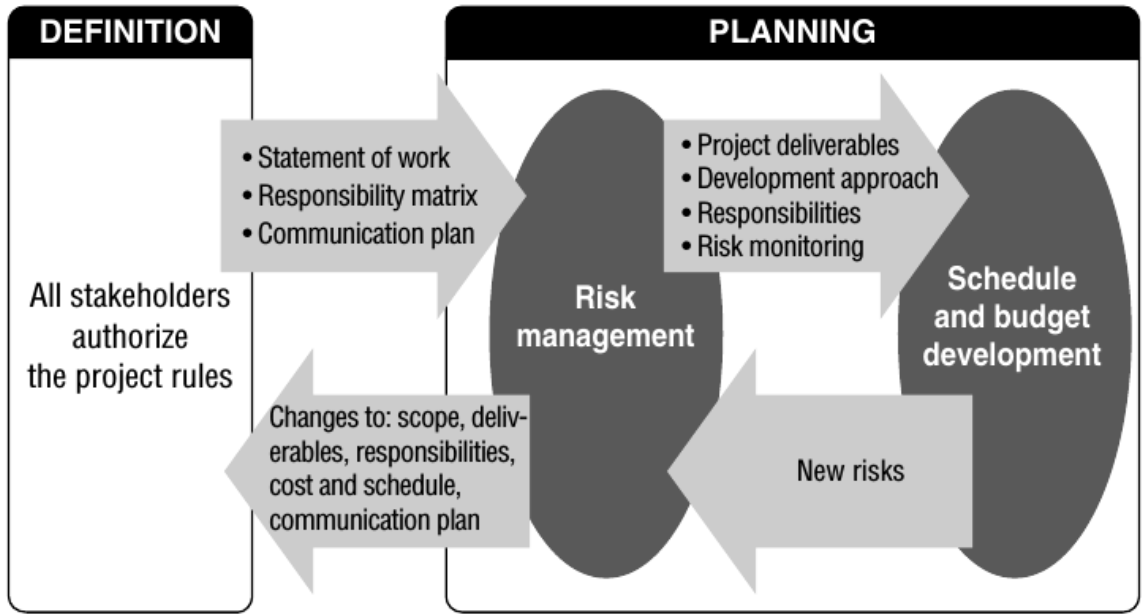
\includegraphics[width=0.9\textwidth]{planning.png}
                \end{center}
            \end{column}
        \end{columns}
    \end{frame}

    \section{Управление рисками}

    \begin{frame}
        \frametitle{Управление рисками}
        \begin{columns}
            \begin{column}{0.4\textwidth}
                \begin{itemize}
                    \item Риск = неопределённость + неприятный исход
                    \begin{itemize}
                        \item Известное неизвестное
                        \item Неизвестное неизвестное
                    \end{itemize}
                    \item Управление рисками~--- первоочередная задача менеджера проекта
                \end{itemize}
            \end{column}
            \begin{column}{0.6\textwidth}
                \begin{center}
                    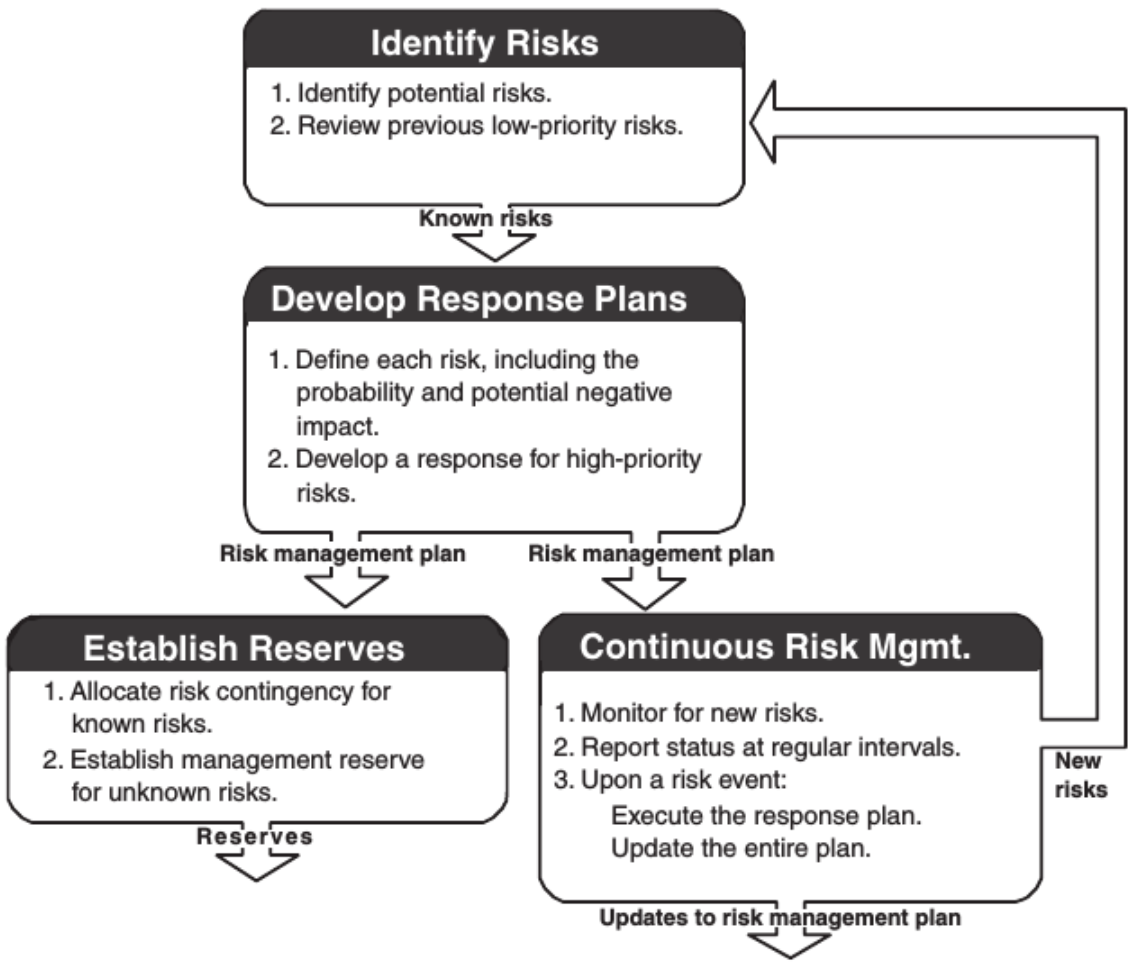
\includegraphics[width=0.95\textwidth]{riskManagementLoop.png}
                \end{center}
            \end{column}
        \end{columns}
    \end{frame}

    \begin{frame}
        \frametitle{Шаг 1: идентификация рисков}
        \begin{itemize}
            \item Получение информации от stakeholder’ов
            \begin{itemize}
                \item Мозговые штурмы
                \item Интервью
            \end{itemize}
            \item Использование прошлого опыта
            \begin{itemize}
                \item Построение профиля рисков
                \item анализ аналогичных проектов
            \end{itemize}
            \item Риски графика работ и бюджета
        \end{itemize}
    \end{frame}

    \begin{frame}
        \frametitle{Шаг 2: разработка стратегии противодействия}
        \begin{itemize}
            \item Определение серьёзности риска
            \begin{itemize}
                \item Описание условий возникновения и последствий
            \end{itemize}
        \end{itemize}
        \begin{columns}
            \begin{column}{0.6\textwidth}
                \begin{itemize}
                    \item Определение вероятности возникновения
                    \begin{itemize}
                        \item Количественные оценки
                        \item Субъективная качественная оценка
                    \end{itemize}
                    \item Определение стратегии снижения возможного урона
                    \begin{itemize}
                        \item Принять
                        \item Избежать
                        \item Переложить на кого-то другого
                        \item Смягчить
                        \item Отслеживать
                        \begin{itemize}
                            \item События-триггеры
                        \end{itemize}
                    \end{itemize}
                \end{itemize}
            \end{column}
            \begin{column}{0.4\textwidth}
                \begin{center}
                    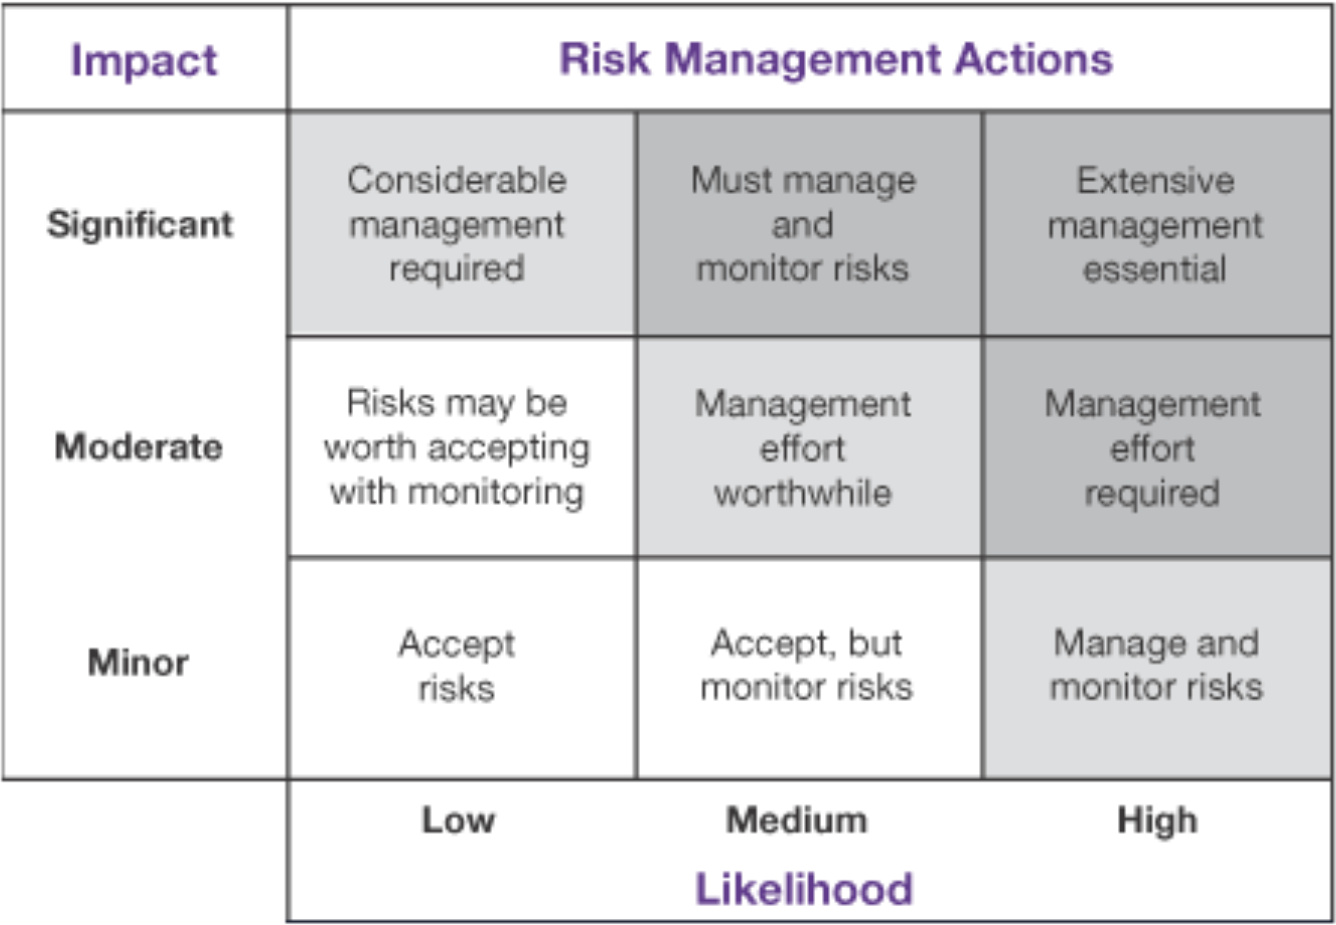
\includegraphics[width=0.95\textwidth]{riskMatrix.png}
                \end{center}
            \end{column}
        \end{columns}
    \end{frame}

    \begin{frame}
        \frametitle{Шаг 3: Создать резервный фонд}
        \begin{itemize}
            \item Противодействие известным рискам
            \begin{itemize}
                \item Определить План Б для каждого отслеживаемого риска
                \item Оценить стоимость Плана Б для каждого риска
                \item Умножить на вероятности и сложить
                \item Согласовать \enquote{разумный} бюджет
            \end{itemize}
            \item А ещё есть неизвестное неизвестное!
            \begin{itemize}
                \item +5-30\% бюджета в зависимости от типа проекта
            \end{itemize}
        \end{itemize}
    \end{frame}

    \begin{frame}
        \frametitle{Шаг 4: Непрерывное управление рисками}
        \begin{itemize}
            \item Поддержание списка рисков
            \item Запланированные переоценки известных рисков
            \item Поиск информации, поиск новых рисков
            \item Анализ резервного фонда
        \end{itemize}
    \end{frame}

    \section{Декомпозиция проекта}

    \begin{frame}{Декомпозиция проекта}
        \begin{center}
            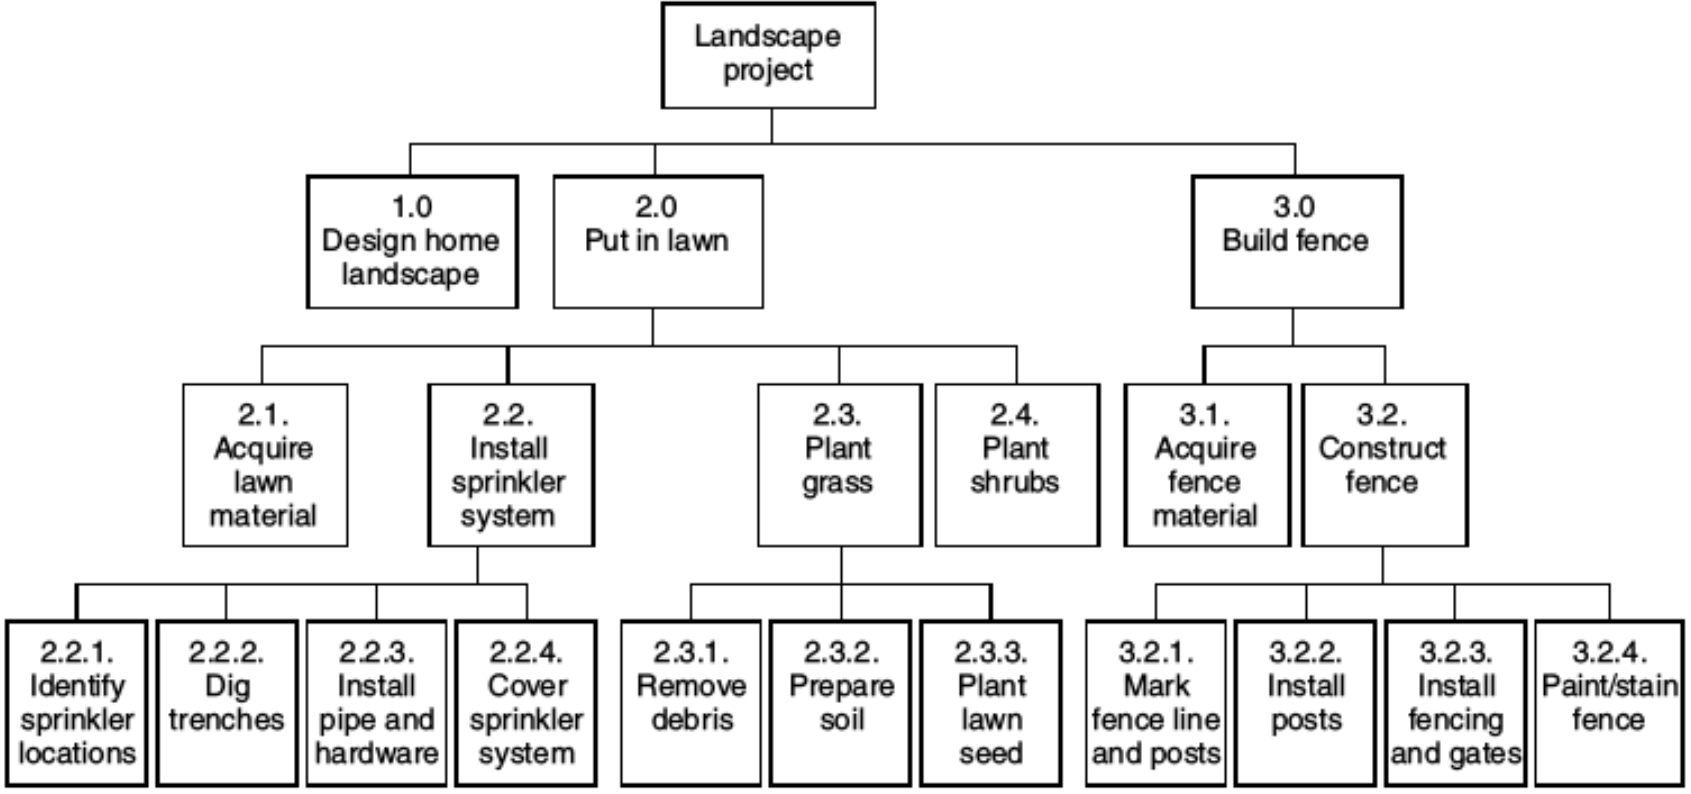
\includegraphics[width=\textwidth]{wbsExample.png}
        \end{center}
    \end{frame}

    \begin{frame}
        \begin{center}
            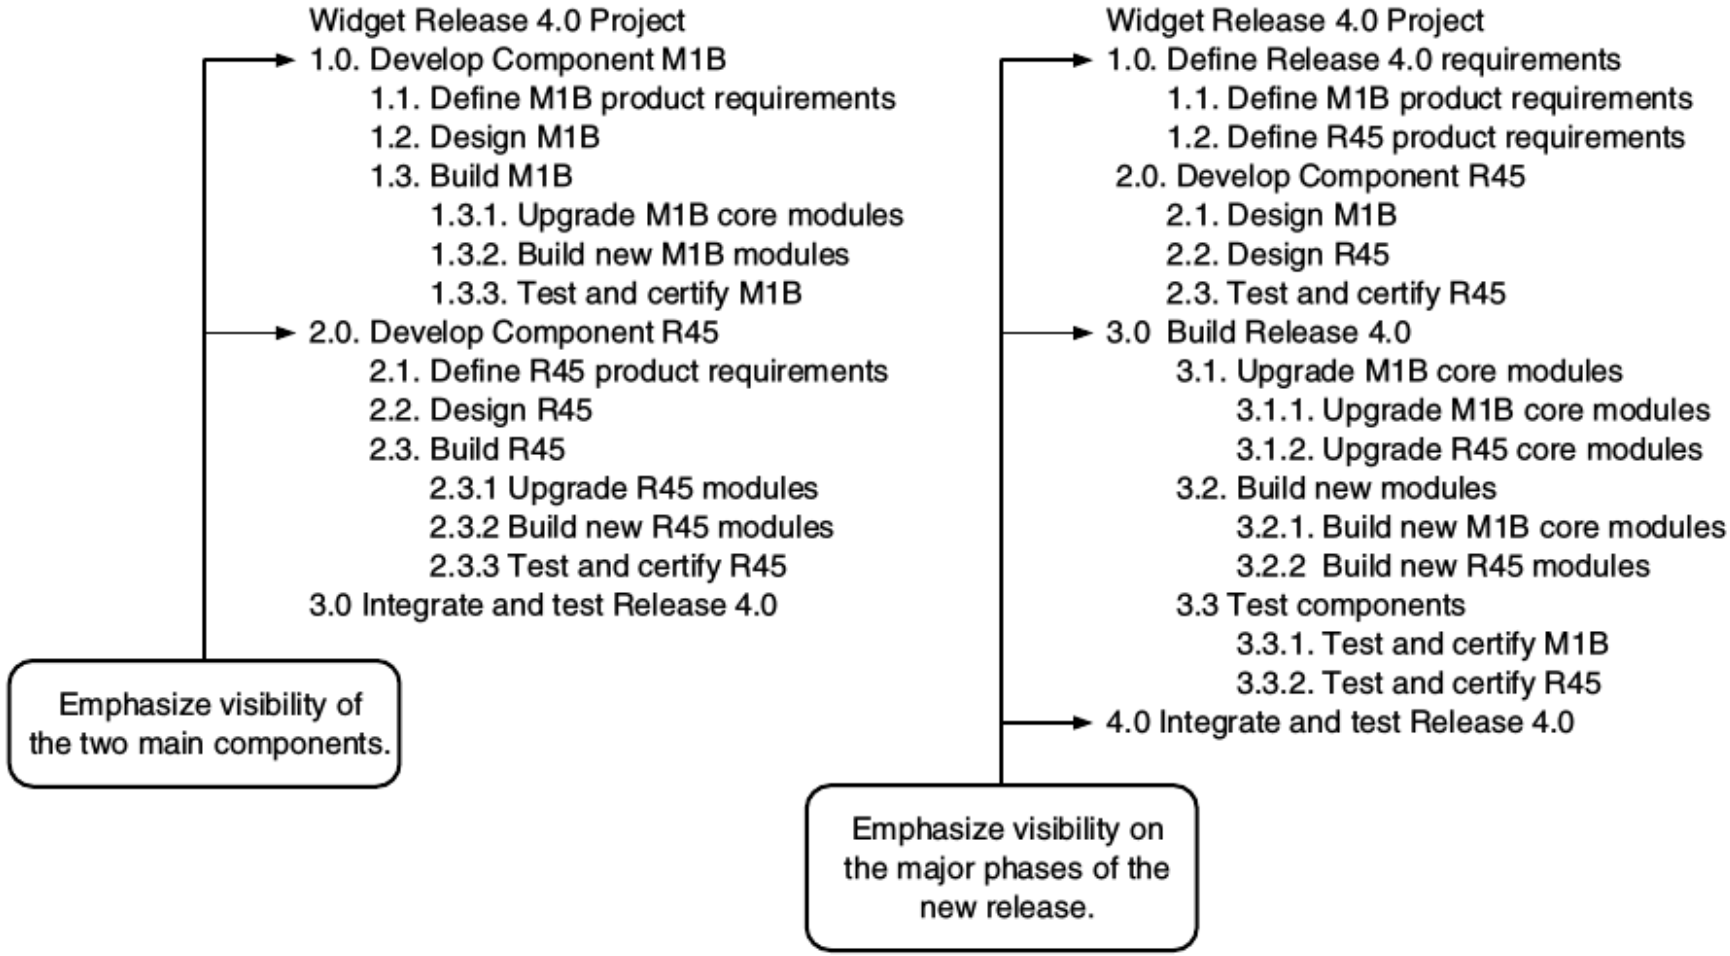
\includegraphics[width=0.9\textwidth]{wbsExample2.png}
        \end{center}
    \end{frame}

    \begin{frame}
        \frametitle{Критерии хорошей декомпозиции}
        \begin{itemize}
            \item Не TODO~--- требуются отчуждаемые артефакты
            \item Полнота разбиения задач
            \begin{itemize}
                \item На всех уровнях сумма объёма дочерних работ в точности равна объёму работы дочернего узла
                \item Отдельные работы друг с другом не пересекаются
            \end{itemize}
            \item Понятность и конкретность задач
            \begin{itemize}
                \item Явный вид деятельности
                \item Явный результат
            \end{itemize} 
        \end{itemize}
    \end{frame}

    \begin{frame}
        \frametitle{Критерии SMART}
        \begin{itemize}
            \item Specific~--- задача должна быть конкретной
            \begin{itemize}
                \item И однозначно пониматься всеми участниками
            \end{itemize}
            \item Measurable~--- задача должна быть измеримой
            \begin{itemize}
                \item KPI, желательно числовые
            \end{itemize}
            \item Achievable~--- задача должна быть достижимой 
            \begin{itemize}
                \item Реальные сроки
                \item Опираться на объективные показатели (предыдущий опыт, средние показатели)
            \end{itemize}
            \item Relevant~--- задача должна быть значимой
            \begin{itemize}
                \item Укладываться в общую стратегию проекта
            \end{itemize}
            \item Time bound~--- задача должна быть ограниченной по времени
            \begin{itemize}
                \item Правило 8/80
            \end{itemize}
        \end{itemize}
    \end{frame}

    \section{Планирование проекта}

    \begin{frame}
        \frametitle{Планирование проекта}
        \begin{enumerate}
            \item Определение целей проекта и требований
            \item Анализ рисков
            \item Декомпозиция проекта
            \item Выявление зависимостей между задачами
            \item Оценка задач
            \begin{itemize}
                \item Методом \enquote{сверху вниз} и \enquote{снизу вверх}
            \end{itemize}
            \item Создание и оценка плана работ
            \item Распределение и оптимизация ресурсов
        \end{enumerate}
    \end{frame}

    \begin{frame}
        \frametitle{Матрица зависимостей}
        \begin{center}
            \begin{tabularx}{\textwidth} { 
                | >{\centering\arraybackslash}X 
                | >{\centering\arraybackslash}X 
                | >{\centering\arraybackslash}X | }
                \hline
                Операция                                  & Непосредственно предшествующие операции & Длительность \\
                \hline
                A. Установка компьютеров                  &~---                                     & 1            \\
                \hline
                B. Протяжка сети                          &~---                                     & 2            \\
                \hline
                C. Настройка сети                         & A, B                                    & 3            \\
                \hline
                D. Установка программного обеспечения     & C                                       & 1            \\
                \hline
                E. Разработка регламента использования ПО &~---                                     & 4            \\
                \hline
                F. Обучение пользователей                 & D, E                                    & 3            \\
                \hline
            \end{tabularx}
        \end{center}
    \end{frame}

    \begin{frame}
        \frametitle{Сетевой график}
        \begin{center}
            \begin{tikzpicture}
                [every path/.style={font=\ssmall}]

                \node[shape=circle,draw=black] (1) at (0,0) {1};
                \node[shape=circle,draw=black] (2) at (2.5,1.5) {2};
                \node[shape=circle,draw=black] (3) at (2.5,-1.5) {3};
                \node[shape=circle,draw=black] (4) at (5,0) {4};
                \node[shape=circle,draw=black] (5) at (8,0) {5};
                \node[shape=circle,draw=black] (6) at (11,0) {6} ;
                
                \path [->](1) edge node[align=center] {A. Установка компьютеров\\ \textit{1 день}} (2);
                \path [->](1) edge node[align=center] {B. Протяжка сети\\ \textit{2 дня}} (3);
                \path [->,dashed](3) edge node[] {} (2);
                \path [->](2) edge node[align=center] {C. Настройка сети\\ \textit{1 день}} (4);
                \path [->](4) edge node[align=center,below=5pt] {D. Установка программного\\ обеспечения\\ \textit{1 день}} (5);
                \path [->](5) edge node[align=center,below=5pt] {F. Обучение\\ пользователей\\ \textit{1 день}} (6);
                \path [->](1) edge[bend right=70] node[align=center,below] {E. Разработка регламента\\использования ПО\\ \textit{1 день}} (5);
            \end{tikzpicture}
        \end{center}
    \end{frame}

    \begin{frame}
        \frametitle{Оценка задач}
        \begin{enumerate}
            \item Длительность
            \begin{itemize}
                \item Календарное время от начала работ до получения конечного результата
                \item Часы, дни, ...
            \end{itemize}
            \item Объём работ
            \begin{itemize}
                \item Абстрактные единицы работы для решения задачи
                \item Человеко-часы, человеко-дни, story points, ...
            \end{itemize}
            \item Конвертация одного в другое
        \end{enumerate}

        $$\textup{Длительность работ} = \frac{\textup{Объём работ}}{\textup{Производительность}}$$
    \end{frame}

    \begin{frame}
        \frametitle{Чем занимаются программисты, когда пишут код}
        \begin{center}
            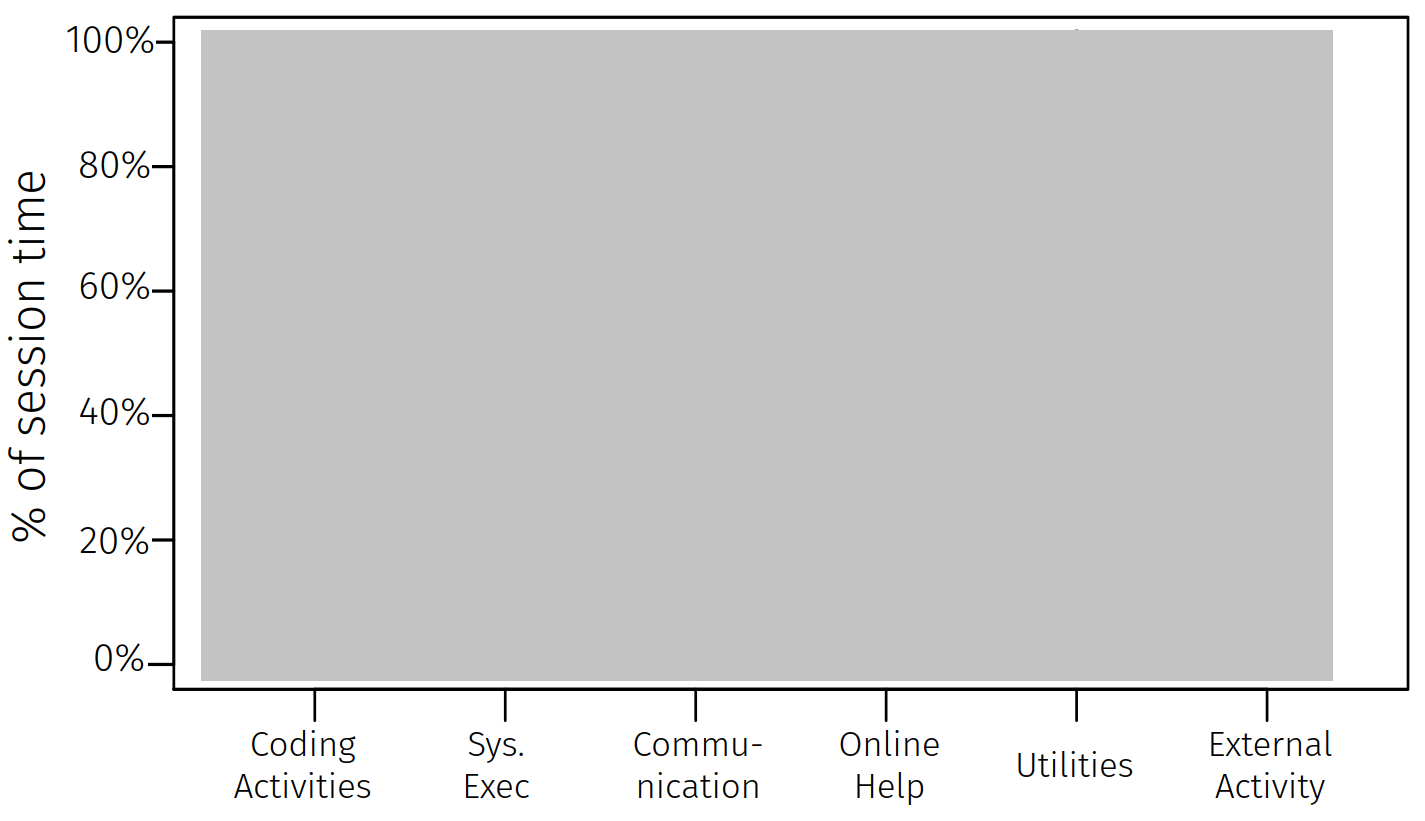
\includegraphics[width=0.95\textwidth]{timeSpentDuringWorkingSessionBlurred.png}
            \attribution{Astromskis et al. Patterns of Developers Behaviour: A 1,000-hour Industrial Study, 2017}
        \end{center}
    \end{frame}

    \begin{frame}
        \frametitle{Чем занимаются программисты, когда пишут код}
        \begin{center}
            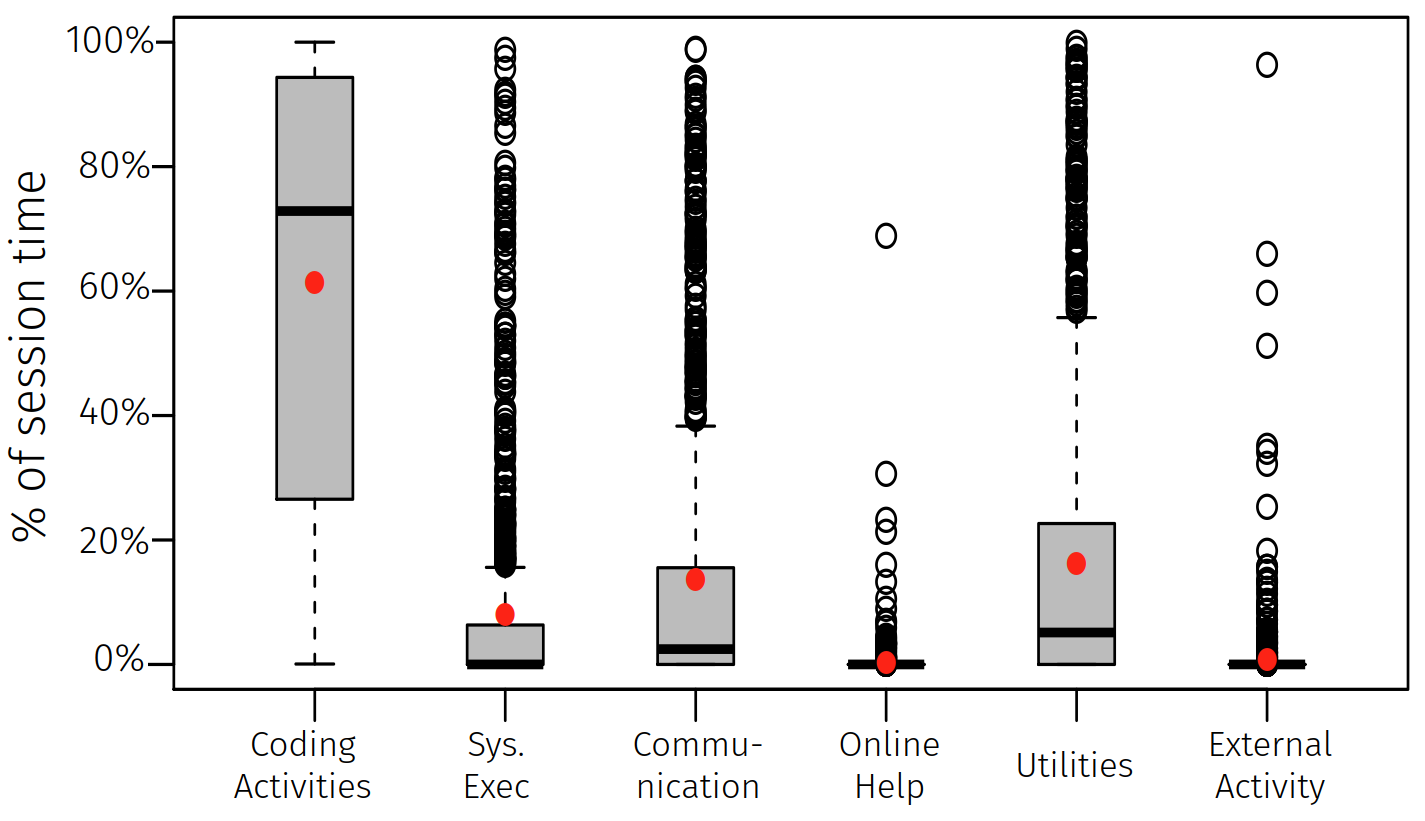
\includegraphics[width=0.95\textwidth]{timeSpentDuringWorkingSession.png}
            \attribution{Astromskis et al. Patterns of Developers Behaviour: A 1,000-hour Industrial Study, 2017}
        \end{center}
    \end{frame}

    \begin{frame}
        \frametitle{Чем занимаются программисты на работе вообще}
        \begin{center}
            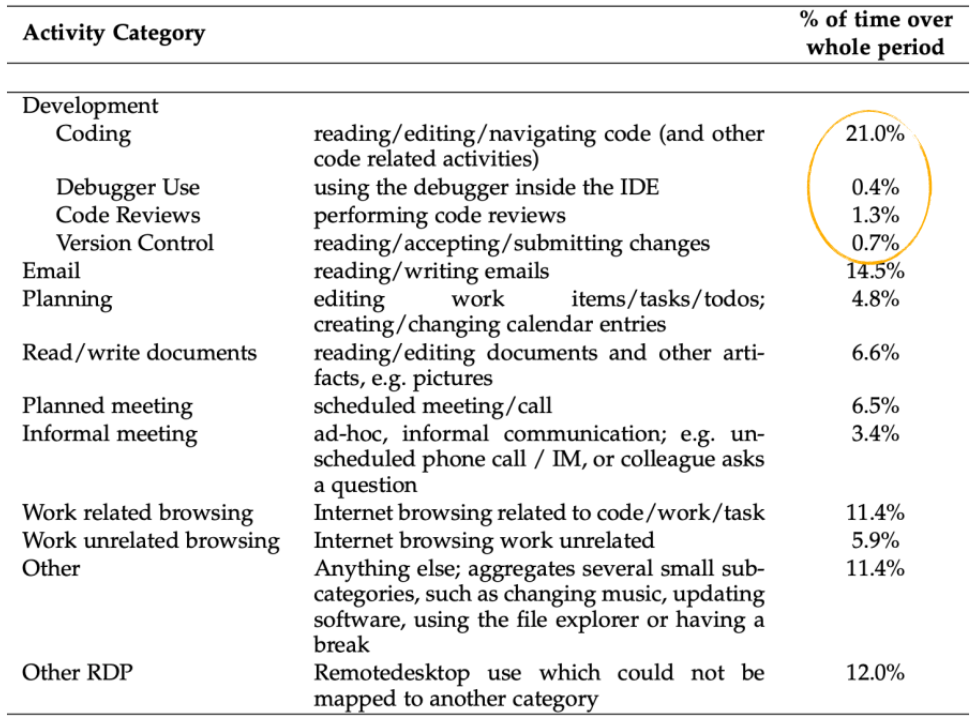
\includegraphics[width=0.7\textwidth]{timeSpentTotal.png}
            \attribution{Meyer et al. The work life of developers: Activities, switches and perceived productivity, 2017}
        \end{center}
    \end{frame}

    \begin{frame}
        \frametitle{Оценка графика работ}
        \begin{itemize}
            \item Прямой проход
            \item Обратный проход
            \item Вычисление резервов
            \item Критический путь
        \end{itemize}
        \begin{center}
            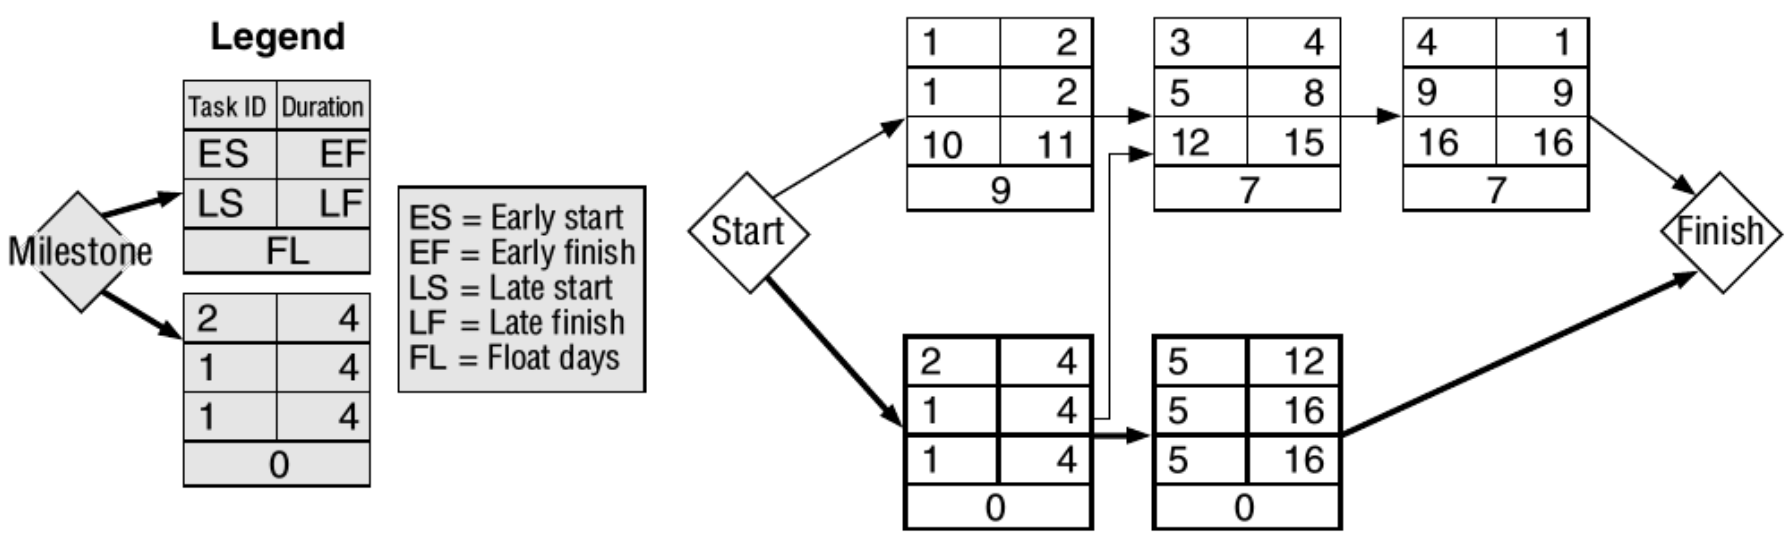
\includegraphics[width=0.95\textwidth]{graphEstimate.png}
        \end{center}
    \end{frame}

    \begin{frame}
        \frametitle{Диаграмма Гантта}
        \begin{itemize}
            \item 1910 год!
            \item Календарный график + зависимости работ
            \item Early start
        \end{itemize}
        \begin{center}
            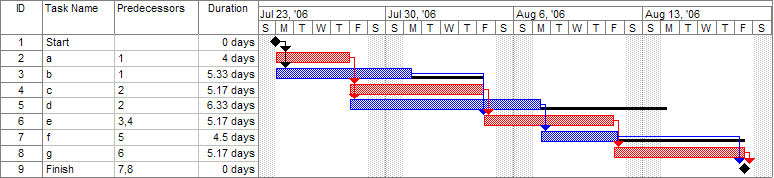
\includegraphics[width=0.95\textwidth]{ganttChart.png}
        \end{center}
    \end{frame}

    \begin{frame}
        \frametitle{Диаграмма Гантта с ресурсами}
        \begin{center}
            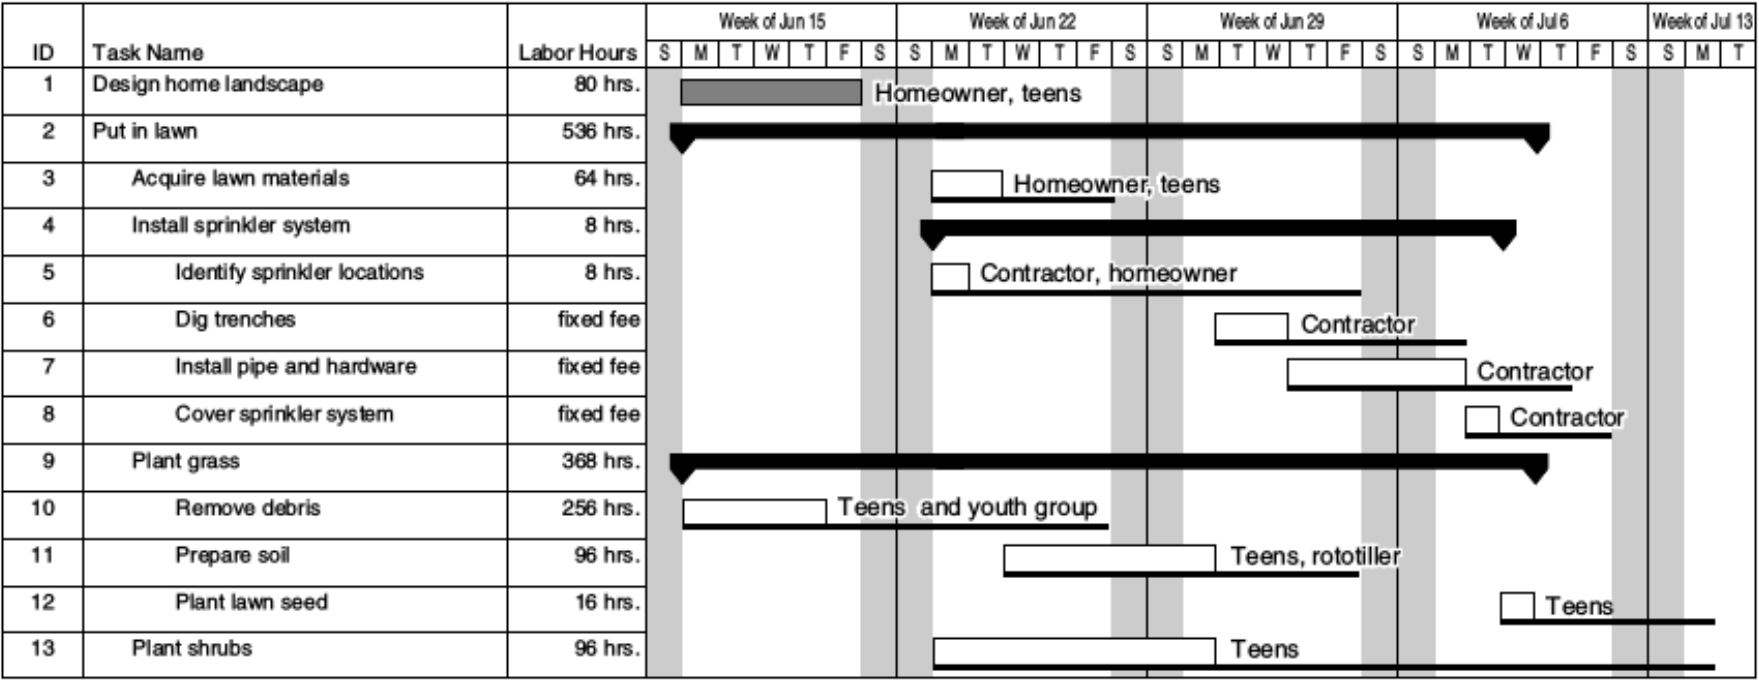
\includegraphics[width=0.95\textwidth]{ganttChartWithResources.png}
        \end{center}
    \end{frame}

    \begin{frame}
        \frametitle{Загруженность ресурсов}
        \begin{center}
            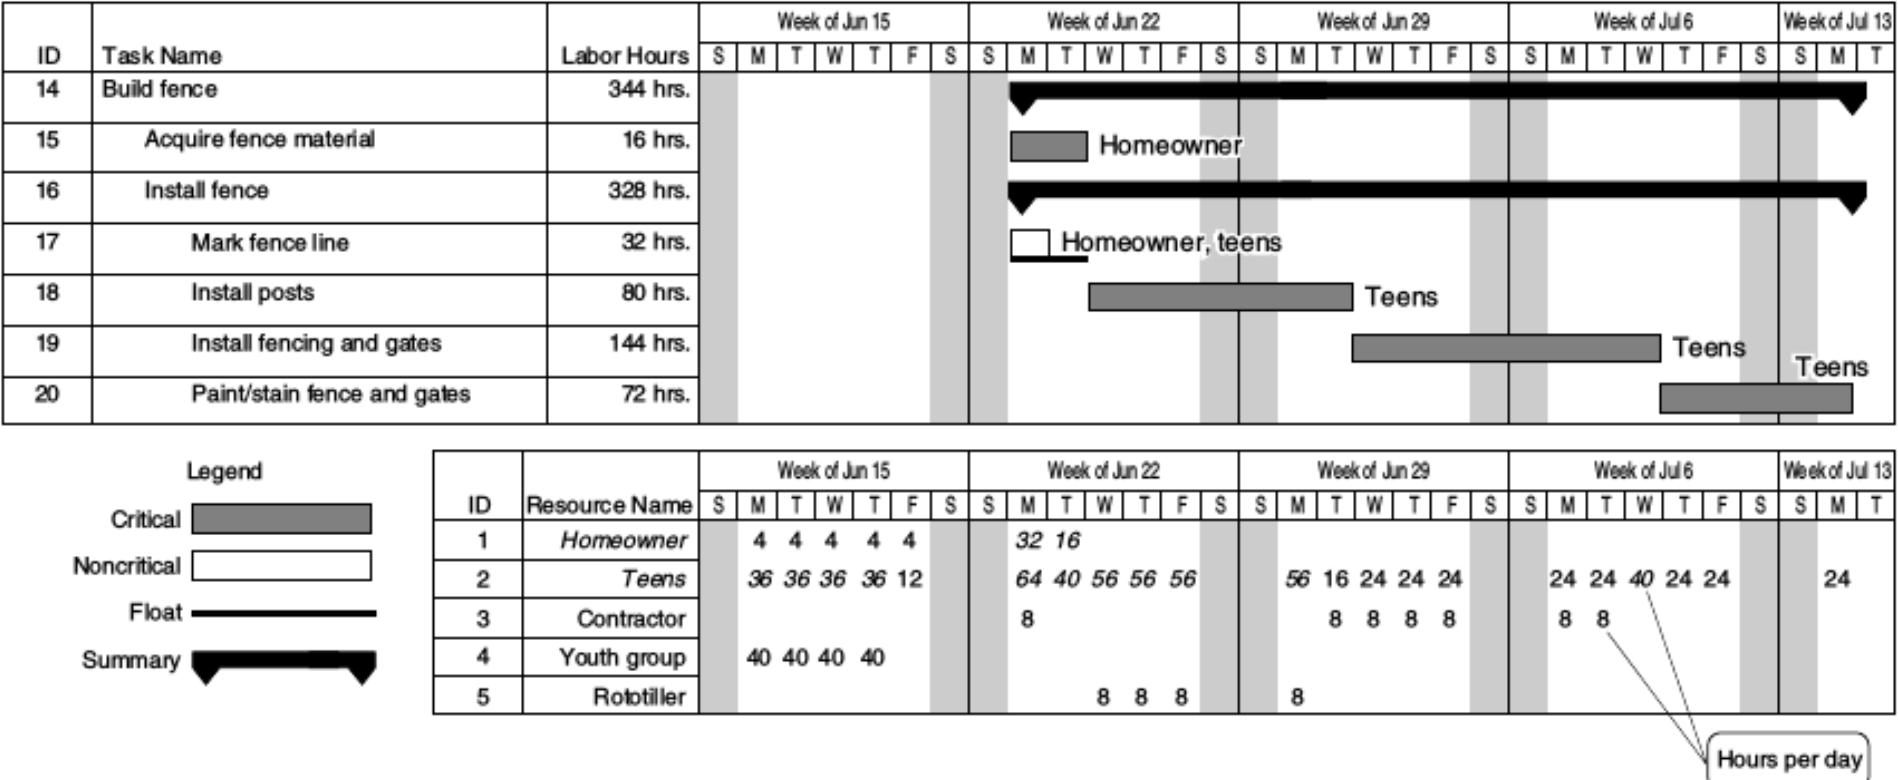
\includegraphics[width=0.95\textwidth]{ganttChartResourceUtilization.png}
        \end{center}
    \end{frame}

    \begin{frame}
        \frametitle{Оптимизация ресурсов}
        \begin{itemize}
            \item Перегруженность и недозагруженность
            \item Оценка ресурсов по начальному графику
            \item Определение и выравнивание пиков
            \item Переоценка задач, перераспределение людей
        \end{itemize}
        \begin{center}
            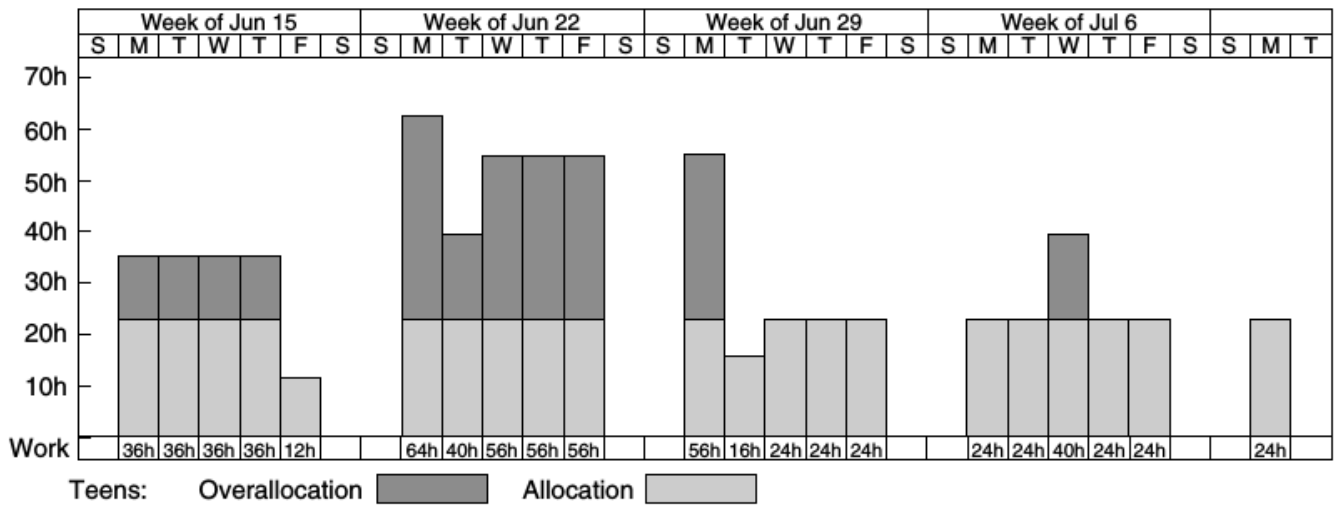
\includegraphics[width=0.7\textwidth]{resourceAllocation.png}
        \end{center}
    \end{frame}

    \begin{frame}
        \frametitle{Планирование денежного потока}
        \begin{center}
            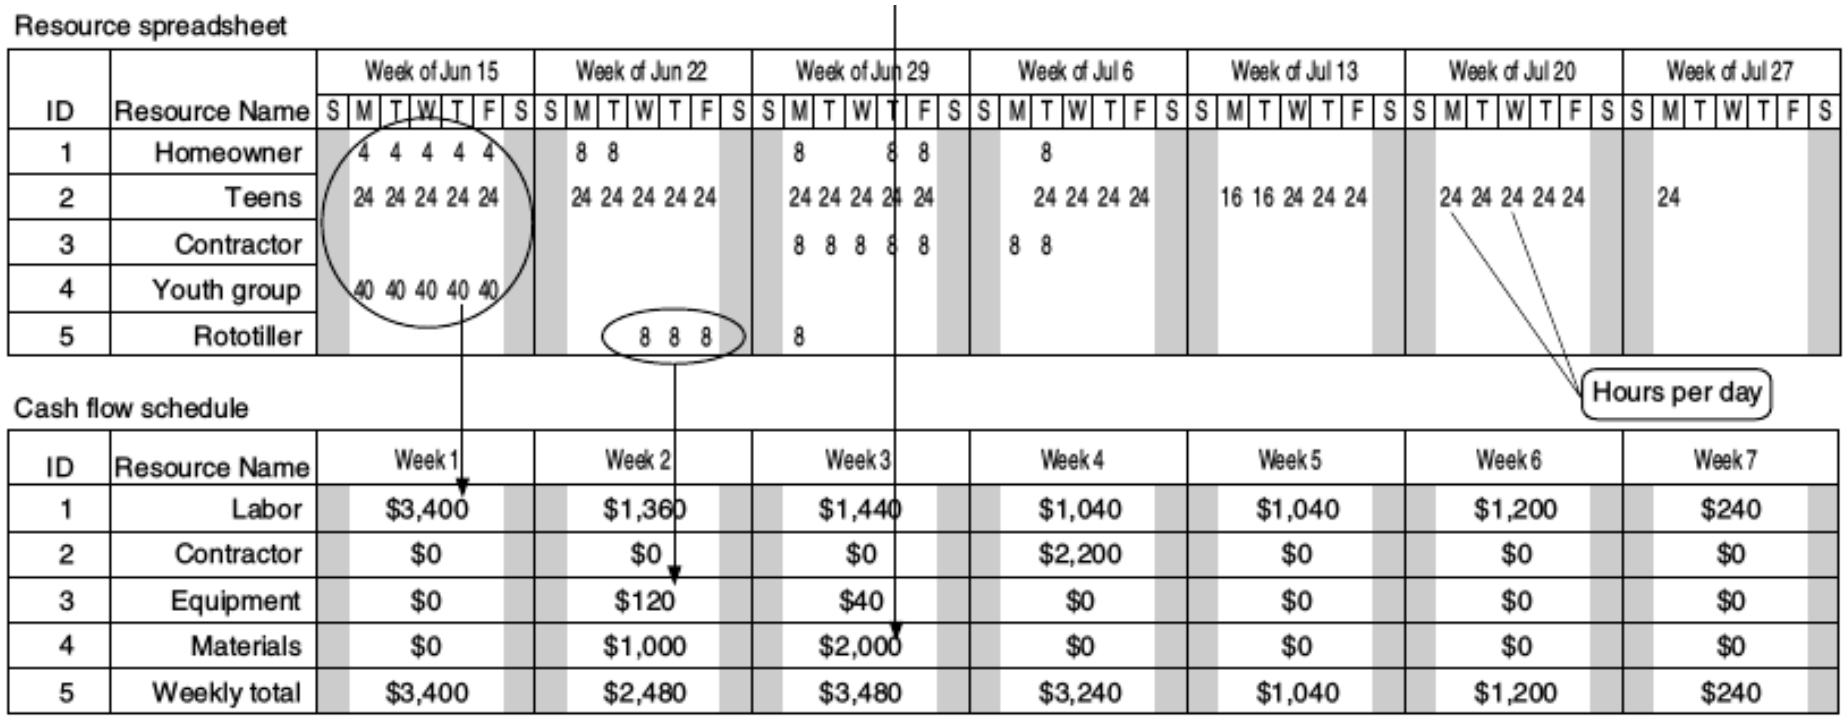
\includegraphics[width=0.95\textwidth]{cashFlow.png}
        \end{center}
    \end{frame}

    \begin{frame}
        \frametitle{Типичные ошибки при оценке проектов}
        \begin{itemize}
            \item Оценку делали не те люди
            \begin{itemize}
                \item Мало опыта, непонимание техник оценивания
            \end{itemize}
            \item Слишком быстрый ответ
            \begin{itemize}
                \item Оценка в условиях недостаточной информации
            \end{itemize}
            \item Забыли про риски и прочие буферы
            \item Забыли налоги
            \item Забыли про расходы на \enquote{административный аппарат}
            \item Забыли про отпуск
            \item Забыли про индексацию зарплат
            \item Забыли про закупки
            \item Политика vs здравый смысл
        \end{itemize}
    \end{frame}

    \begin{frame}
        \frametitle{Уровни детальности оценки}
        \begin{itemize}
            \item \enquote{Оценка в лифте}
            \item Оценка при выборе проекта
            \item Детальная оценка
        \end{itemize}
        \begin{center}
            
\includegraphics[width=0.7\textwidth]{dilbertEstimation.png}
        \end{center}
    \end{frame}

\end{document}
